\chapter{Introduction}\label{ch:intro}


\textcolor{red}{somewhere we should add a note about the intended audience. In paritcular I want to be throrough and include all relevant details and derivations that I wish I had when I started.}



What we want:

1. Introductory paragraph(s) describing the goal of the dissertation

Current methods for water and air quality analysis are limited in two key ways:
1. Insufficient quantity of data at relevant spatial, spectral, and temporal
resolutions
2. Simulating full physical dynamics is often computationally infeasible to
provide actionable insights fast enough to enable human action/intervention.



- The rapid pace of global change increasingly endangers human health and well-being
and threatens environmental health and stability
- Continued advancements in low-cost, mobile sensing have dramatically increased
our ability to characterize the environment at spatial and temporal resolutions
relevant to human-scale interactions
- Additionally, a plethora of satellite missions have been recently launched (or
will soon be) which promise to provide petabytes of multi-spectral imagery
- However, the data provided by these systems are often limited to specific
physical quantities (e.g. reflectances) which are only indirectly related to water quality and air
quality parameters which we actually care about
- To make sense of these data, one can apply physical models which relate
measurements to parameters of interest
- However, these models are limited by the physics \textit{as we currently
  understand it} making it challenging to account for as yet undiscovered
relationships impacting the data 
- Additionally, simulating the dynamics of physical systems at scale demands 
significant computational resources limiting real-time applicability.
- For example, ECMWF meteorological forecasts are provided a (add spatial and
temporal resolution) despite the fact the many studies across the scientific
literature suggest relevant spatial scales between 0-1 km and temporal scales at
the order of 10 seconds for air quality.
- Machine learning offers a suite of data-driven methods to take advantage of
large datasets to extract meaningful relationships between 


% Amidst the rapid pace of global change, accurately assessing water and air quality is crucial for protecting the environment and safeguarding human health and well-being.

% Traditional monitoring methods are often insufficient to capture the complex and
% dynamic nature of these environmental systems, necessitating the development of
% advanced data collection and modeling techniques.


\section{Dissertation Goals}


The goal of this dissertation is to advance physical sensing in service of society by demonstrating the use of new techniques from physics-based machine learning on a variety of real world data sets. Towards this end, this work presents a collection of case studies utilizing both supervised and unsupervised machine learning techniques in a variety of contexts together with physical sensing to produce actionable environmental insights. The applications of this research apply widely across many scientific domains including remote sensing, time series analysis, air quality, chemical kinetics, and data assimilation.




\section{Summary of Original Contributions}

\subsection{Publications}
- Robot team supervised 1
- Robot team unsupervised GTM
- Robot team unsupervised GSM
- HAVOK models for PM outlier detection and short-term foractasting

\subsection{Datasets}
\subsection{Code}










%\section{Motivation}
\section{Water Quality}


\section{Air Quality}
Research into air quality began in
earnest in the mid-20th century driven by growing concerns over the impact of
pollution, industrial emissions, and urban smog on public health. In the US, the
Clean Air Act of 1963 accelerated research efforts by empowering the federal
government with authority to address air pollution standards. However, at the
time  


- Multiple components which contribute to overall air quality
- Gasses are a big one
- Describe all of the parameters that go into the Air Quality Index
- We focuse

- Prabuddha et al. combine remote sensing observations for aerosol optical depth
with meteorological data to predict ground level PM 2.5 using machine learning
together with ground based-sensors \cite{prabuddha-pm-satellite}
- Average US values exceeded 9 $\mu g/m^3$ standard 20\% of the time with the
eastern US and California exceeding the limit over 50\% of the time during the
sampling period from Jan. 2020 to June 2023.

\subsection{What is Particulate Matter}

\subsection{Environmental Impact}

\textcolor{red}{include a picture of fog/haze}

\subsection{Human Impact}




\section{Physical Sensing}

The successful application of machine learning methods demands comprehensive, carefully curated data sets. In order for our modeling efforts to be successful, it is critical that we capture the subtle nuances of the phenomena we wish to describe. In this chapter, we outline the various physical sensing approaches used throughout this dissertation, all of which are part of a broader effort in the MINTS-AI laboratory at the University of Texas at Dallas. MINTS-AI is an acronym for Multi-Scale Multi-Use Integrated Intelligent Interactive Sensing in Service of Society for Actionable Insights. An graphical overview of the MINTS-AI sensing paradigm is outlined in Figure \ref{fig:mints-ai}.

\begin{figure}[!hbt]
  \centering
  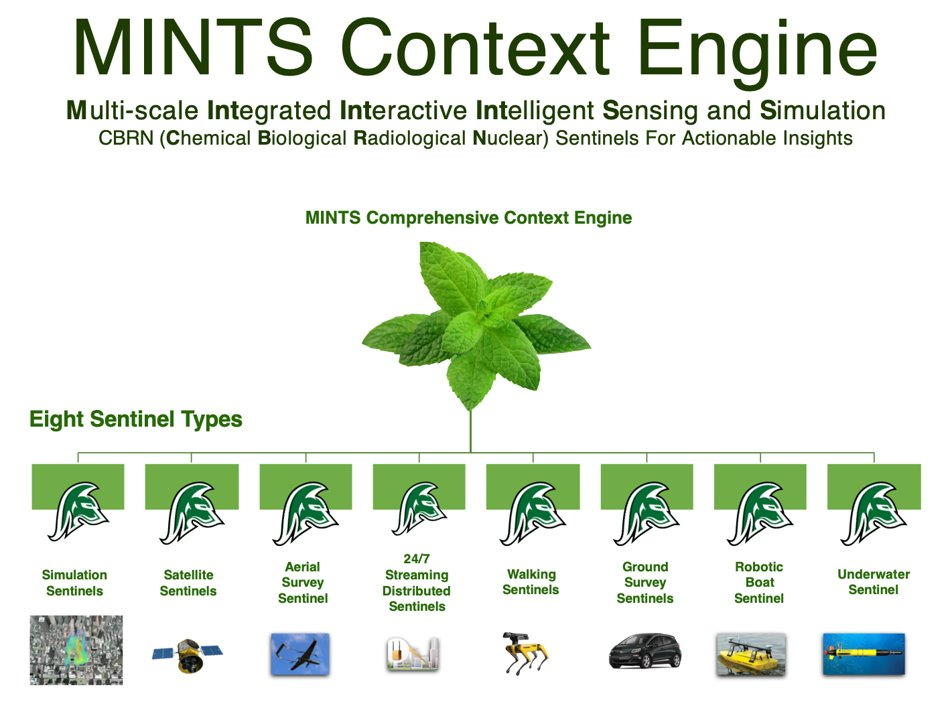
\includegraphics[width=0.8\textwidth]{introduction/MINTS-sentinels.jpg}
  \caption{The MINTS-AI context engine is a sensing paradigm composed of flexible sensing sentinels spanning from remote sensing data products to autonomous robots and ground survey vehicles.}
  \label{fig:mints-ai}
\end{figure}

Of the variety of sensing sentinels listed above, this dissertation is primarily concerned with three key applications. The first is a team of autonomous robotic vehicles which we refer to as the \textit{robotic team}. The second is a network of distributed streaming sentinels comprised of low-cost air quality sensors. The third describes a reference sensor chamber for air quality evaluation which we use to develop a \textit{simulation sentinel}.






\section{Machine Learning}

- The Role of Machine Learning in the Era of Big Data

Big data in the physical sciences
Comment on the annual data volumes produced by
\begin{itemize}
  \item LANDSAT
  \item Sentinel
  \item CERN
  \item James Webb
  \item SDO AIA
  \item Medical Imaging (MRI, CT scans, etc...)
\end{itemize}

What is machine learning

Use of machine learning in the physical sciences

\begin{itemize}
  \item Remote sensing (inter-instrument calibration, classification, object identification, change monitoring via the NDVI and similar indices, etc.)
  \item Protein Folding
  \item Drug discovery
  \item Surrogate modeling (i.e. for PDE solvers - now very popular at NVIDIA)
\end{itemize}


\subsection{Supervised and Unsupervised ML}


\subsection{Physics-based Machine Learning}

Successful physical theories are predictive, explainable, and quantifiable (i.e.
uncertainty can be characterized). Most machine learning tasks involve abstract
data for which this can be challenging. A physics-based machine learning
approach involves model selection, uncertainty quantification, physical
reasonableness, etc..


The general problem of ML is hard with when no structure is assumed on data (include example of pit bull or potato)

For situations involving data from physical sensors describing real systesm, physics tells us there are underlying rules which govern the dynamics of real systems

When applying ML we should therefore place a high value on physics-based models, i.e. machine learning models tailord for the specific physical system, rather than generic abstract algorithms. This is important in all stages of the ML pipeline from feature selection (Robot team supervised), dimensionality reduction (i.e. the latent space of the GTM and GSM), model selection, model evaluation, etc. In summary:

\begin{itemize}
  \item Prefer interpretable models (e.g. deicsion trees) to black boxes
  \item Prefer probabilistic models (e.g. GTM vs SOM) to deterministic models (all data has uncertainty and no model is perfect)
  \item Prefer models which incorporate prior knoweldge of the physical system such as dynamical laws, symmetries, natural constraints, etc. This is specifically known as \textbf{physics-informed} machine learning or \textbf{scientific machine learning}  (SciML).
\end{itemize}



\section{Actionable Insights}

Combining physical sensing with machine learning methods allows us to \textit{put science in action} in order to drive positve societal outcomes.


\section{Dissertation Overview}

